\documentclass{article} % For LaTeX2e
\usepackage{nips12submit_e,times}
%\documentstyle[nips12submit_09,times,art10]{article} % For LaTeX 2.09

\usepackage{amsmath,amssymb,amsthm,amsfonts,comment}
\usepackage{graphicx}\graphicspath{{figures/}}
\usepackage[small,labelfont=bf]{caption}
\usepackage[square]{natbib}
\usepackage{color}
\usepackage{epstopdf}
\newcommand{\theHalgorithm}{\arabic{algorithm}}

%% our math environment
\def\[#1\]{\begin{align}#1\end{align}}

\newcommand{\defn}[1]{{\bf #1}}

\newcommand{\defas}{:=}
\newcommand{\given}{\mid}

\newcommand{\Naturals}{\mathbb{N}}
\newcommand{\Rationals}{\mathbb{Q}}
\newcommand{\Reals}{\mathbb{R}}
\newcommand{\cS}{\mathcal{S}}
\newcommand{\st}{\,:\,}
\newcommand{\RInts}{\mathcal{I}_\Rationals}
\newcommand{\BSets}{\mathcal{B}_\Reals}
\newcommand{\grad}{\bigtriangledown}

%% our math environment
 
\newtheorem{thm}{Theorem}
\newtheorem{cor}[thm]{Corollary}
\newtheorem{lem}[thm]{Lemma}
%\newtheorem{definition}{Definition}

\title{Optimal independence tests for Bayesian Networks}

\author{
\And
Coauthor \\
Affiliation \\
Address \\
\texttt{email} \\
\AND
Coauthor \\
Affiliation \\
Address \\
\texttt{email} \\
\And
Coauthor \\
Affiliation \\
Address \\
\texttt{email} \\
\And
Coauthor \\
Affiliation \\
Address \\
\texttt{email} \\
(if needed)\\
}

% The \author macro works with any number of authors. There are two commands
% used to separate the names and addresses of multiple authors: \And and \AND.
%
% Using \And between authors leaves it to \LaTeX{} to determine where to break
% the lines. Using \AND forces a linebreak at that point. So, if \LaTeX{}
% puts 3 of 4 authors names on the first line, and the last on the second
% line, try using \AND instead of \And before the third author name.

\newcommand{\fix}{\marginpar{FIX}}
\newcommand{\new}{\marginpar{NEW}}

%\nipsfinalcopy % Uncomment for camera-ready version

\begin{document}


\maketitle

\begin{abstract}

\end{abstract}


\section{Introduction}
Learning Bayesian networks for general distributions is
intractable task \cite{chickering1996learning}. However, in practise 
for distributions appearing in real data, still we are able to 
recover Bayesian network structure. This implies that real data
distribution has some special properties, which simplify process
of structure recovery. This process is almost always
based on computation local statistics, and then 
reasoning about global structure \cite{jaakkola2010learning, tsamardinos2006max}. 
Local statistics describe
complexity (e.g. number of parameters in case of BIC), and 
level of independence between nodes (e.g. mutual information tests, 
conditional independence tests). 
We focus in this work on improvement of independence tests by 
learning it for CPDs present in data.


We consider parameterized family of independence tests. 
Before inferring about structure of Bayesian network, we tune classifier 
predict independence or dependence on CPDs present in data. 
This way, we obtain highly sensitive independence test, which
fires on dependence or independence phenomenas present in our data. 


\section{Related work}
Independence tests used in Bayesian networks
\begin{itemize}
\item \cite{schafer2005empirical} Here they learn a Gaussian Graphical Model (GGM) using estimates of the partial correlation matrix. 
\item \cite{opgen2007correlation} Here they learn an approximate causal structure on gene expression based on full-order partial correlation (as an approximation to lower-order partial correlation that is called for theoretically for a Bayesian network).
\item \cite{tsamardinos2006max} MMHC algorithm.  They use a test based on what is called the $G^2$ statistic (asymptotically distributed as $chi^2$) and they also talk about a couple other independence tests that we may want to look into.
\end{itemize}

There has been extensive research in area of scoring functions for
Bayesian networks. This step is critical to recover no-complete graph structure.
Without any scoring function, log-likelihood term would force optimization
to choose fully connected graph. There have been proposed few regularizations (scoring functions)
to address this problem. One most widely used is Bayesian Information Criterion (BIC) \cite{schwarz1978estimating}.
Variety of such scoring functions calculate dependency between nodes conditioned on
potential parents \cite{de2006scoring}. Usual measures of dependency are
based on mutual information, conditional independence test, or 
are fully Bayesian. Fully Bayesian methods assume probability 
distribution over CPDs of independent variables,
and dependent variables.




We should discuss:
\begin{itemize}
\item LL (Log-likelihood) (1912-22)
\item MDL/BIC (Minimum description length/Bayesian Information Criterion) (1978)
\item AIC (Akaike Information Criterion) (1974)
\item NML (Normalized Minimum Likelihood) (2008)
\item MIT (Mutual Information Tests) (2006)
\end{itemize}
Use in Bayesian networks \cite{schafer2005empirical}

Existing independence tests:
\begin{itemize}
\item Pearson's $\chi$-squared.  The problem is the null hypothesis is independence, but independence is what we're trying to show.
\end{itemize}

\cite{margaritis2003learning}

\section{Independence testing} TODO : Wojciech (give a pass to Arthur Gretton)
Independence tests have to decide if random variables are independent.
Samples of this random variables gives us indirect access to the conditional probability
distribution (CPD), which decides on independence. However, samples itself
provide only empirical estimate on conditional probability distribution. 
Moreover, manifold \ref{fig:ind} of independent CPDs among all possible CPDs
have a measure zero. 


\begin{figure}[h]
\centering
\includegraphics[width=0.55\linewidth]{img/independence_surface.eps}
\caption{The manifold of independence for binary distributions. The simplex represents all possible joint distributions over two binary variables.  a, b, and c are three of the four entries in the joint distribution table, and the simplex is formed by the constraint that all entries must be positive and sum to one.  The manifold corresponds to the set (of measure zero) of independent distributions.}
\label{fig:ind}
\end{figure}

\subsection{Curse of conditioning}

\subsection{Partial correlation}

\subsection{Kernelized partial correlation}

\section{Experiments}

\subsection{Classification of Synthetic CPDs}
We generated distributions from toy Bayesian networks.

\begin{figure}[h]
\centering
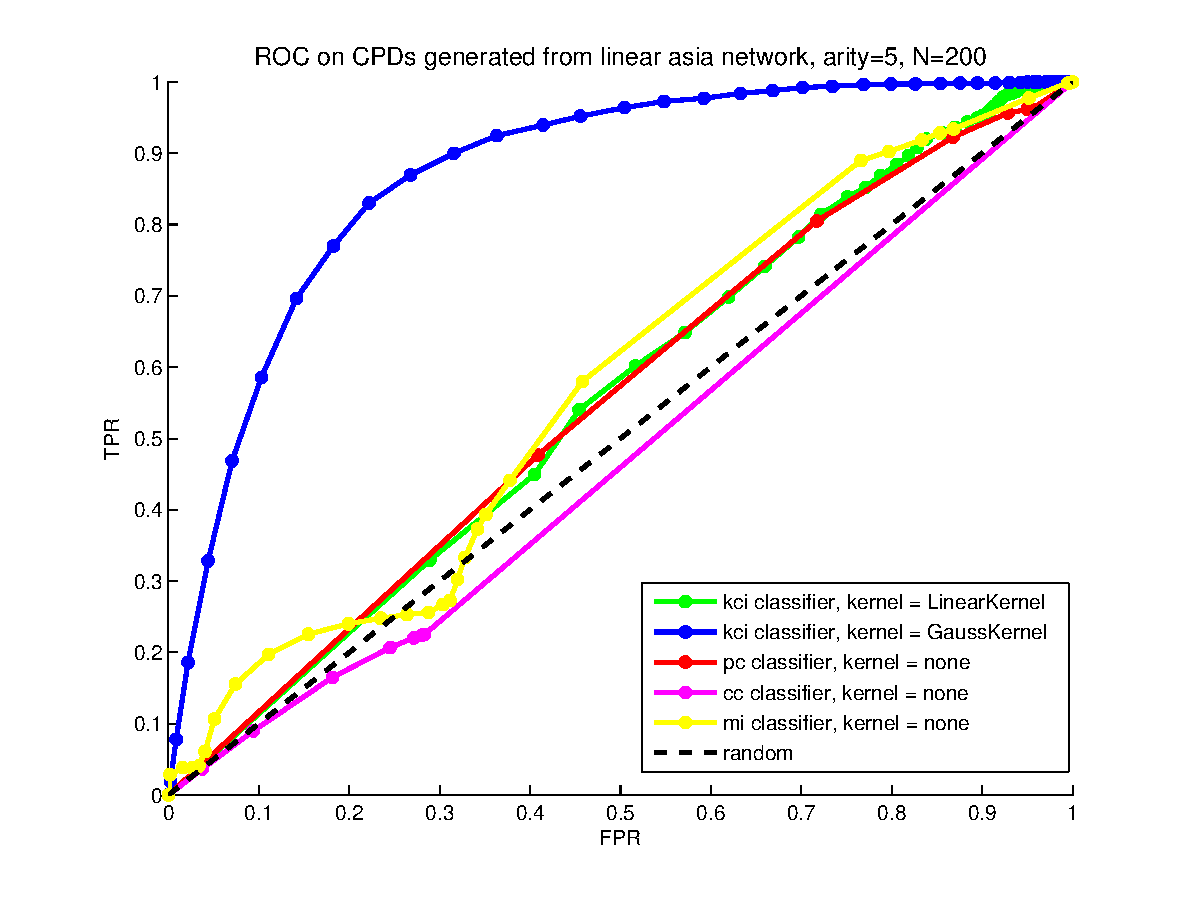
\includegraphics[width=0.55\linewidth]{img/roc_full_random_arity5.eps}
\caption{A}
\end{figure}

\begin{figure}[h]
\centering
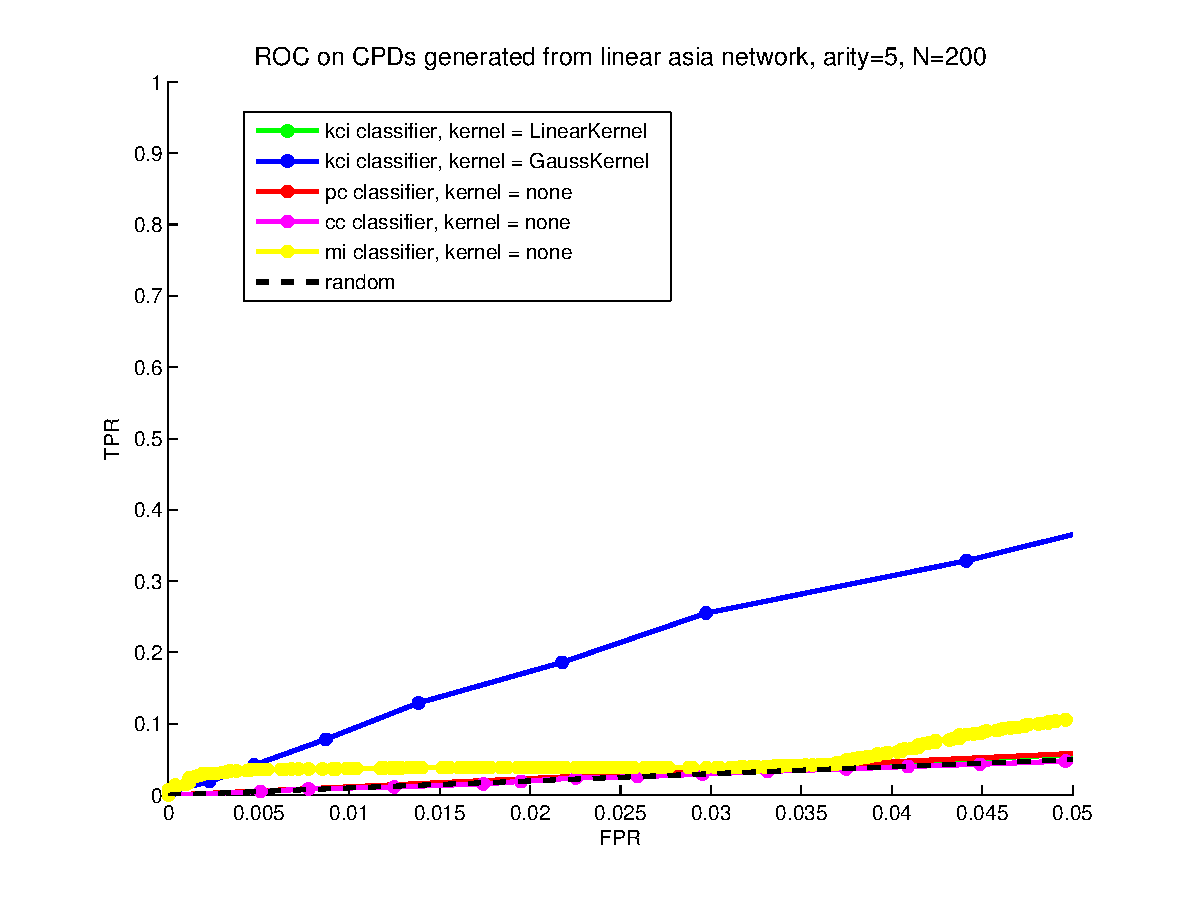
\includegraphics[width=0.55\linewidth]{img/roc_partial_random_arity5.eps}
\caption{A}
\end{figure}
\subsection{Classification of CPDs from Gene Expression}

\subsection{Synthetic Bayesian networks}

\subsection{Gene expression data}

\section{Discussion}

\begin{small}
%\renewcommand\bibname{References}
\bibliographystyle{abbrvnat}
%\bibliographystyle{authordate1}
%\bibliographystyle{amsnomr}
\bibliography{bibliography}
\end{small}

%\appendix
%\include{appendix}

\end{document}
